\documentclass{article}

\usepackage[a4paper, margin=2cm]{geometry}

\usepackage[utf8]{inputenc}
\usepackage[czech]{babel}
\usepackage{fvextra}
\usepackage{csquotes}
\usepackage{expl3}

\usepackage{parskip}
\usepackage[hidelinks, unicode, pdfusetitle]{hyperref}

\usepackage{float}
\usepackage{minted}
\usepackage{graphicx}
\graphicspath{{images}}

\title{34-3-3 Jízda tramvají}
\author{Benjamin Swart}

\begin{document}

\maketitle

\section{Matematika}

Prvním krokem bude pro každou sílu v seznamu vypočítat interval směrů, kterými může být Jirka v okamžik jejího působení otočen. Je jedno, jestli jsme otočeni ve směru působení síly nebo ve směru jemu opačném, takže platné úhly mají periodu 180°. Tyto intervaly budeme reprezentovat jako dvojice čísel. Pokud sílu ustojíme, ať jsme orientovaní jakkoliv, tak ji přeskočíme.

\begin{figure}[H]
    \centering
    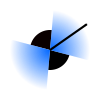
\includegraphics[width=5cm]{angles.pdf}
\end{figure}

Nyní se snažíme najít cestu s nejmenším počtem horizontálních přesunů v tomto "bludišti": (Černé čáry představují intervaly, kde by Jirka spadl.)

\begin{figure}[H]
    \centering
    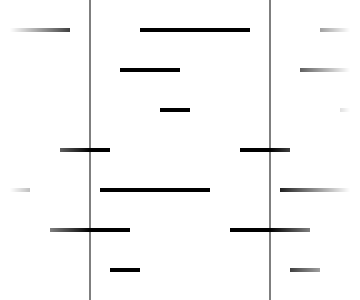
\includegraphics[height=8cm]{waterfall/empty.pdf}
\end{figure}

\section{Limitace na cesty}

Hned ze začátku si můžeme všimnout několika faktů. Zaprvé je zbytečné se otáčet, pokud následující sílu ustojíme se současnou rotací. Sice bychom se potenciálně příště nemuseli otočit tak daleko, ale v součtu se stejně otočíme stejně daleko. Naopak existuje šance, že se budeme muset otočit zpátky. Zadruhé si můžeme všimnout, že pokud se otočit musíme, tak podobně nemá smysl se otáčet na některou stranu dále, než je potřeba, abychom následující sílu ustáli.

To nám problém výrazně zjednoduší: Dokud ve výše uvedené mapě nenarazíme na zeď, pokračujeme dál bez otočení. Pokud na zeď narazíme, tak se stačí rozhodnout, jestli se otočíme doleva nebo doprava. Mapa všech možných tras vytvoří jakýsi vodopád:

\begin{figure}[H]
    \centering
    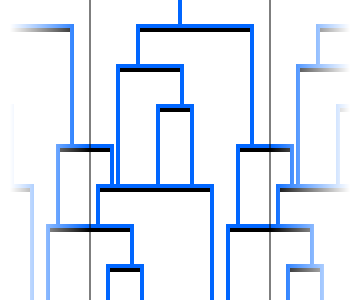
\includegraphics[height=8cm]{waterfall/full.pdf}
\end{figure}

\section{Generace vodopádu}

Tento vodopád můžeme snadno generovat a zároveň v něm hledat nejkratší cestu.

Vytvoříme červeno-černý strom a vložíme do něj Jirkovu počáteční orientaci dohromady s minimálním součtem velikostí rotací potřebných k jejímu dosažení (tj. 0). Budeme ho řadit podle úhlu orientace.

Poté postupně procházíme jednotlivé zdi v bludišti. V červeno-černém stromu můžeme snadno jedním nebo dvěma průchody najít všechny \enquote{proudy}, které se o zeď zastaví. Asymptotická složitost této operace je \(O(log(n)*m)\), kde \(n\) je počet proudů ve stromě a \(m\) je počet nalezených proudů. Pokud zeď žádný proud nezastaví, pokračujeme s příští. Pokud však nějaké proudy najdeme, tak do stromu přidáme dva nové proudy, jeden pro levou a jeden pro pravou stranu zdi. Pro každý proud musíme vypočítat vzdálenost od původní orientace. Tu určíme tak, že projdeme nalezené proudy, sečteme jejich uloženou vzdálenost s vzdáleností od daného kraje zdi a z těchto součtů vezmeme minimum. Nakonec ze stromu ukončené proudy odstraníme.

Až projdeme všechny zdi, tak projdeme proudy, které nám ve stromě zůstaly. Mezi nimi najdeme ten s nejnižší vzdáleností a tu vypíšeme.

Pokud chceme vypsat i potřebnou sekvenci otočení, můžeme si ke každému proudu uložit i odkaz na jeho \enquote{předchůdce}, proudy odstraněné ze stromu ponechat po zbytek běhu programu v paměti a nakonec projít trasu pozpátku jako u Dijkstrova algoritmu.

\section{Složitost}

Všechny relevantní operace s červeno-černým stromem běží v \(O(log(n))\) vzhledem k jeho velikosti. Proudů bude celkem nanejvýš \(2 * m + 1\), kde \(m\) je počet sil. Proto všechny operace běží v \(O(log(n))\) vzhledem k počtu sil. Každý proud přidáme, najdeme a odstraníme právě jednou. Celý algoritmus tedy běží v \(O(n*log(n))\), alespoň pokud dokážeme provádět operace na reálných číslech v konstantním čase. Paměťová složitost je \(O(n)\)

\appendix
\newpage
\section{O hroších}

To, že jsou hroši hnědí \\
To přeci všichni už vědí \\
Co však nesklízí žádné díky \\
Jsou hroší znalosti informatiky \\
Hroší dovednosti v oblasti IT \\
Jsou však, jak mi víme, znamenité \\
Takový hroch je s trochou času schopen \\
Napsat traveling salesman v \(O(n*log(n))\)

\end{document}